%\documentclass[handout]{beamer} % use this to disable \pause commands
\documentclass{beamer}
%
% Choose how your presentation looks.
%
% For more themes, color themes and font themes, see:
% http://deic.uab.es/~iblanes/beamer_gallery/index_by_theme.html
%
\mode<presentation>
{
  \usetheme{default}      % or try Darmstadt, Madrid, Warsaw, ...
  \usecolortheme{default} % or try albatross, beaver, crane, ...
  \usefonttheme{default}  % or try serif, structurebold, ...
  \setbeamertemplate{navigation symbols}{}
  \setbeamertemplate{caption}[numbered]
  \setbeamertemplate{footline}{% 
    \hfill% 
    \usebeamercolor[fg]{page number in head/foot}% 
    \usebeamerfont{page number in head/foot}% 
    \insertframenumber%
    %\,/\,\inserttotalframenumber
    \kern1em\vskip2pt% 
  }
} 

\usepackage[english]{babel}
\usepackage[utf8x]{inputenc}
\usepackage{pdfcomment}
\usepackage{fancyvrb}
\usepackage{tabularx}

\newcommand{\pdfnote}[1]{\marginnote{\pdfcomment[icon=note]{#1}}}
\newcommand\mydots{\hbox to 1em{.\hss.\hss.}}

\title[Your Short Title]{Concurrent Programming with\\Actors and Microservices}
\author{Maximilian Irro}
\date{Diplomprüfung\\12.11.2018}

\begin{document}

\begin{frame}
  \titlepage
\end{frame}

% Uncomment these lines for an automatically generated outline.
\begin{frame}{Outline}
  \tableofcontents
\end{frame}

% ###################################################################

\section{Overview: Concurrency, Actors, Microservices}

% ###################################################################

\begin{frame}{Forms of Concurrent Execution}

\begin{itemize}
  \item \textbf{Pseudo-Simultaneous}: in alternation on a single CPU
  \item \textbf{Parallel}: truely simultaneous on several CPU cores
  \item \textbf{Distributed}: several host machines
\end{itemize}

\end{frame}

% ###################################################################

\begin{frame}{Actor Model}

\begin{itemize}
  \item Theoretically well-known constructs
  \item Receive and process messages (asynchronous, passiv)
  \item One message at a time
  \item Encapsulate state exclusively
  \item Concurrent execution through runtime
  \item Single-threaded semantics
\end{itemize}

\end{frame}

% ###################################################################

\begin{frame}{Microservices Paradigm}

\begin{itemize}
  \item Complex functionality: composition of several \textit{services}
  \item Microservice: small, independent executable
  \item \glqq Small\grqq{} size $\rightarrow$ in it's \textit{scope of responsibility}
  \item Dedicated operating system processes
  \item Communicate via message passing channels
%  \item Network-based communication $\rightarrow$ distribution
\end{itemize}

\end{frame}

% ###################################################################

\section{Research Questions \& Contributions}

% ###################################################################

\begin{frame}{Research Questions}

\begin{table}
  \begin{tabularx}{\textwidth}{lX}                                                                                                                    \\[10pt]%
    \textbf{RQ1} & Why do actors and microservices qualify for programming concurrency?                                                               \\[10pt]%
    \textbf{RQ2} & How do the actor and the microservice model facilitate concurrent execution?                                                       \\[10pt]%
    \textbf{RQ3} & What are the expressive capabilities of actors and microservices regarding concurrent programming concerns?                        \\[10pt]%
    \textbf{RQ4} & How does the performance of actors and microservices compare in a multi-core environment relative to a concurrent system scenario?
  \end{tabularx}
\end{table}

\end{frame}

% ###################################################################

\begin{frame}{Demarcation of Research Area}

\pause

\begin{center}
  \begin{figure} 
    \includegraphics[width=\textwidth]{graphics/topics-venn.pdf} 
  \end{figure}
\end{center}

\end{frame}

% ###################################################################

\begin{frame}{Selected Capabilities}

\begin{itemize}
  \item \textbf{Encapsulation} \\%
        Isolation (Shared/ Mutable State), Persistence/IO, Cohesion, Coupling, Independence
  \item \textbf{Communication} \\%
        Communication Styles, Message Routing
  \item \textbf{Concurrent Execution} \\%
        Conception of Conc. Exec., Distribution, Location Transparency, Fairness, Resource Consumption, Notion of Time
  \item \textbf{Scalability and Modularity} \\%
        Forms (Vertical, Horizontal, Load), Dynamic Reconfiguration, Extensibility, Technology Diversity
  \item \textbf{Integration of Actors and Microservices}
\end{itemize}

\end{frame}

% ###################################################################

\begin{frame}{Contributions}

\begin{itemize}
  \item Designed a non-trivial concurrent system scenario \\%
        $\rightarrow$ Actor and microservice implementation
  \item Compared programming of concurrency
  \item Describe interrelations $\rightarrow$ filled a gap in the literature
  \item Capability evaluation $+$ efficiency benchmark
\end{itemize}

\end{frame}

% ###################################################################

\section{Implementation}

% ###################################################################

\begin{frame}{Implementation: Domain-specific Search Engine}

\pause

\begin{columns}
  \begin{column}{0.47\textwidth}
    \begin{itemize}
      \item Gateway (G) 
      \item CatalogStore (C)
      \item Updater (U)
      \item Web Crawler (W)
      \item Parser (P)
      \item IndexStore (I)
      \item Searcher (S)
    \end{itemize}
  \end{column}
  \begin{column}{0.5\textwidth}
    \begin{figure} 
      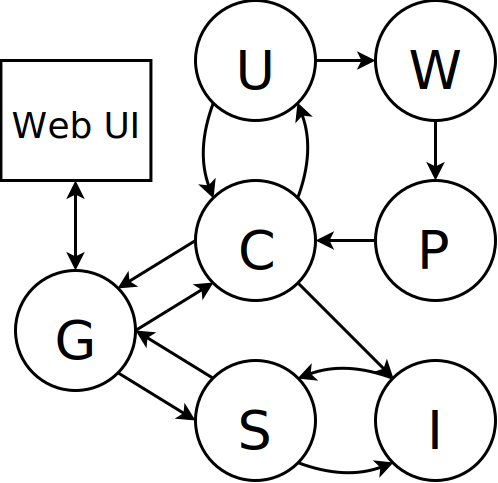
\includegraphics[width=0.7\textwidth]{graphics/interaction-model.png} 
      \caption{Interaction Model}
    \end{figure}
  \end{column}
\end{columns}

\end{frame}

% ###################################################################

\begin{frame}{Implementation: Subsystems \& Processing Pipelines}

\begin{figure} 
  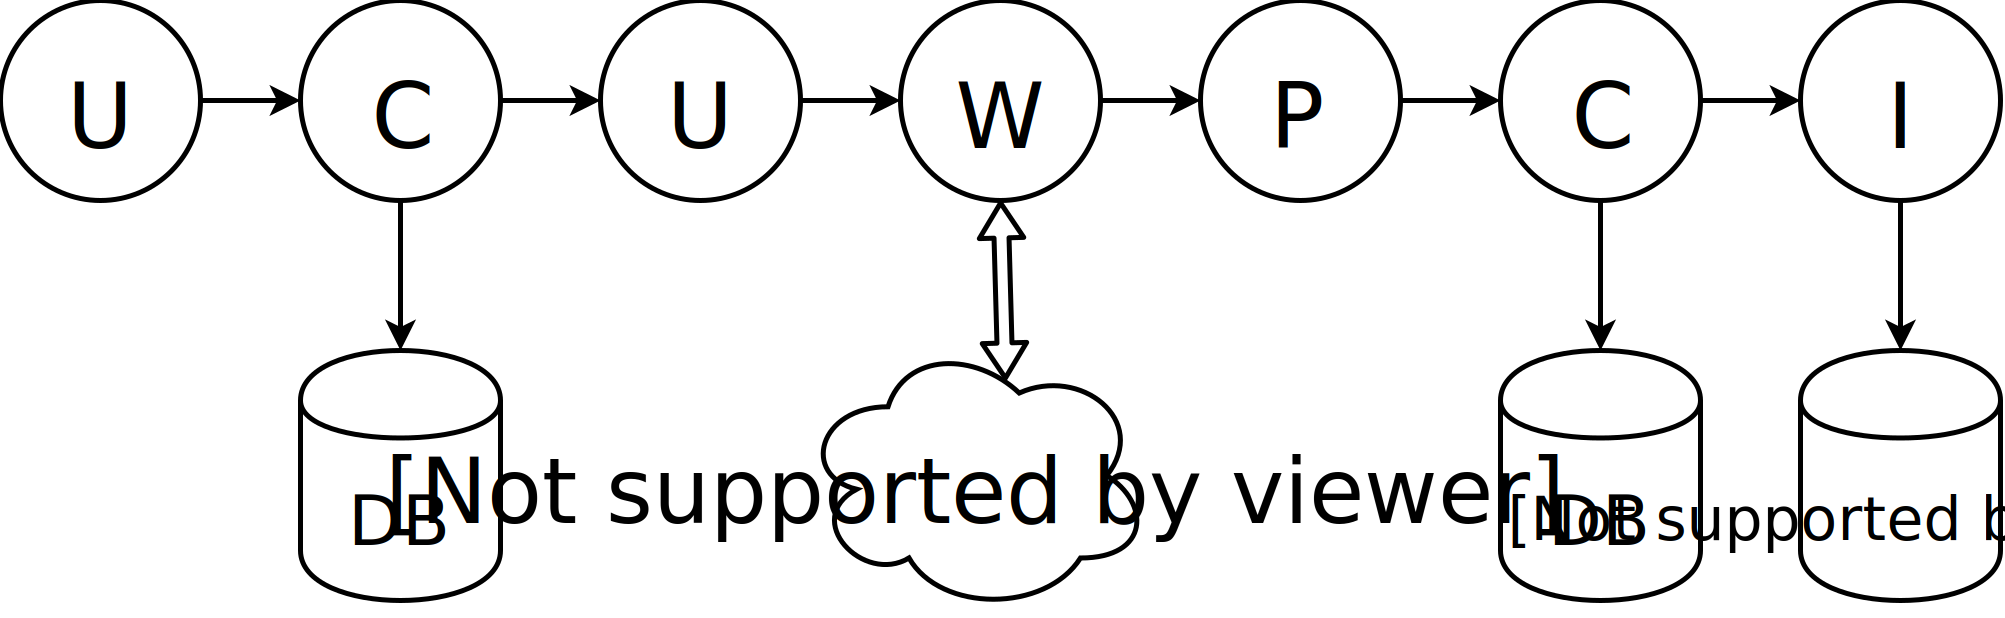
\includegraphics[width=0.77\textwidth]{graphics/pipeline-indexing.png} 
  \caption{Indexing Pipeline}
\end{figure}

\begin{figure} 
  
\includegraphics[width=0.65\textwidth]{graphics/pipeline-retrieval.png} 
  \caption{Retrieval Pipeline}
\end{figure}

\end{frame}

% ###################################################################

\begin{frame}{Implementation: Technology Stacks}

\begin{itemize}
  \item JVM based
  \item Actor variant: Akka
  \item Microservice: Spring Boot $+$ Spring Cloud
\end{itemize}

\end{frame}

% ###################################################################

\section{Benchmark Results}

% ###################################################################

\begin{frame}{Software Artifact Analysis}

\begin{table}
  \begin{tabular}{l|r|r|r|r}
    \textbf{Artifact} & \textbf{LoC} & \textbf{sJAR (KB)} & \textbf{fJAR (KB)} & \textbf{Up (s)}  \\ \hline
    Akka monolith     & 4487         & 1004.3             & 76 775.1           & 5.5              \\ \hline
    CatalogStore (MS) & 1838         & 56.1               & 89 225.8           & 14.6             \\ \hline
    IndexStore (MS)   & 724          & 23.8               & 83 518.2           & 8.8              \\ \hline
    Searcher (MS)     & 656          & 22.2               & 81 754.4           & 8.1              \\ \hline
    Web Crawler (MS)  & 716          & 23.5               & 83 517.9           & 9.2              \\ \hline
    Parser (MS)       & 703          & 24.2               & 83 519.1           & 8.6              \\ \hline
    Registry (MS)     & 334          & 9.9                & 90 699.7           & 9.4              \\ \hline
    Gateway (MS)      & 889          & 30.5               & 83 655.1           & 9.7              \\ \hline
    Updater (MS)      & 693          & 23.9               & 83 518.3           & 8.7              \\ \hline
  \end{tabular}
\end{table}

\begin{itemize}
  \item $\sum\mbox{LoC}(\mbox{MS}) = 6553$, about 46 \% larger
\end{itemize}

\end{frame}

% ###################################################################

\begin{frame}{Artifact Memory Consumption}

Memory consumption of the executable artifact VMs in the indexing phase:

\begin{center}
  \begin{figure} 
    \includegraphics[width=0.5\textwidth]{graphics/eval-index-mem.pdf} 
  \end{figure}
\end{center}

\end{frame}

% ###################################################################

\begin{frame}{Overall Processing Time: Indexing Subsystem}

Benchmark results for the overall processing time of the indexing subsystem:

\begin{center}
  \begin{figure} 
    \includegraphics[width=0.5\textwidth]{graphics/eval-index-overall.pdf} 
  \end{figure}
\end{center}

\end{frame}

% ###################################################################

\begin{frame}{Overall Processing Time: Retrieval Subsystem}

Benchmark results of the overall processing time for the retrieval subsystem:

\begin{center}
  \begin{figure} 
    \includegraphics[width=0.5\textwidth]{graphics/eval-search-rtt-overall.pdf} 
  \end{figure}
\end{center}

\end{frame}

% ###################################################################

\section{Conclusion \& Implications}

% ###################################################################

\begin{frame}{Conclusion \& Implications}

\begin{itemize}
  \item \textbf{Same} capabilities regarding concurrent programming concerns
  \item \textbf{Different} strategies $+$ trade-offs
  \item Actors: more efficient, less resource consumption
  \item Microservices: more independent, more interaction freedom \\%
        $\rightarrow$ benefit from actor principles 
\end{itemize}

\end{frame}

% ###################################################################

\begin{frame}{}

\vspace{1cm}
\begin{center}
  \texttt{</presentation>}
\end{center}

\end{frame}

% ###################################################################

\begin{frame}{Supplemental: Semi-Synchronous Communication in Akka}

Comparison of the benchmark results for the retrieval subsystem using either delegation or futures for request/response communication in the Akka:

\begin{center}
  \begin{figure} 
    \includegraphics[width=0.5\textwidth]{graphics/eval-search-comparison-akka-delegation-future.pdf} 
  \end{figure}
\end{center}

\end{frame}

% ###################################################################

\begin{frame}{Supplemental: State Encapsulation vs. Isolation}

\begin{itemize}
  \item Microservice: process memory boundaries
  \item Actors (on the JVM):
  \begin{itemize}
    \item Visibility $+$ Accessibility $\rightarrow$ information hiding
    \item Reference types $+$ pass-by-value $\rightarrow$ immutability
    \item Coding conventions required
  \end{itemize}
\end{itemize}

\end{frame}

% ###################################################################


\end{document}

